\chapter{The GEM and CSC Data Acquisition Systems}
\label{chap:II-2-daq}

  The installation of GEM detectors in CMS and the integration with the CSCs require the development of a new DAQ system for the GE1/1 project. The understanding of the structure of both the GEM and CSC readout chains as well as the common CMS central DAQ is of importance in the scope of this thesis. To this end, all three systems are presented in details in the sections that follow. \\

  \section{The GE1/1 Data Acquisition System}

    The architecture of the GE1/1 DAQ system is represented in Figure \ref{fig:II-2-daq-gem-system}. It is divided into two sectors: the on-detector electronics on the left in charge of the managment of the detector, and the off-detector electronics on the right responsable for the data handling and the connection to the central DAQ. The two sectors are separated by a few douzen meters and connected through optical fibres. \\

    \begin{figure}[h!]
      \centering
      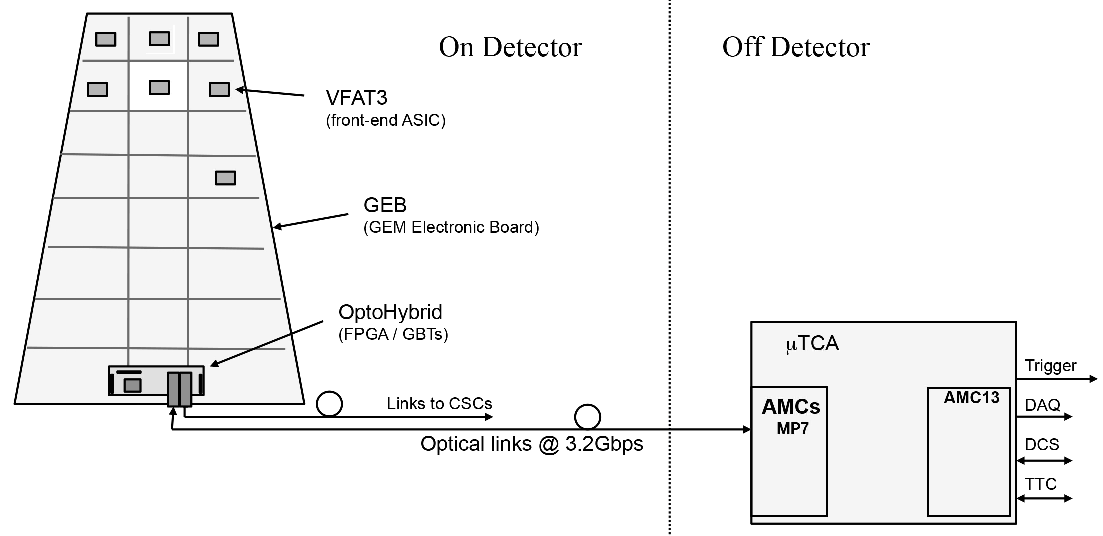
\includegraphics[width=0.7\textwidth]{img/II-2-daq/gem-system.pdf}
      \caption{??? \cite{Colaleo:2021453}.}
      \label{fig:II-2-daq-gem-system}
    \end{figure}

    The on-detector electronics focuses on the control and readout of the VFAT3 Application Specific Integrated Circuit (ASIC) which connects to the strips of the chamber and digitizes the data. The GEM Electronics Board (GEB), on which the VFAT3s are plugged in, then routes the signals to the OptoHybrid (OH) which acts as concentrator board and communication relay for the 24 VFAT3s. The communication with the off-detector system is performed through the GigaBit Tranciever (GBT) chipset and the Versatil Link installed on the OH. Both projects are led by CERN and provide radiation hard tools for LHC experiments. \\

    On the off-detector side, the Micro Telecommunications Computing Architecture (microTCA, MTCA, or $\mu$TCA) \cite{PICMG} crate standard is used to power and monitor the Advanced Mezzanine Cards (AMCs) which provide the ressources to communicate with the on-detector electronics. Links from multiple OHs are concentrated on one MP7 AMC which formats the data and transfers it to the CMS AMC13 mezzanine. The AMC13 is the link between the microTCA crate and the central DAQ of CMS which provides the clocking, trigger, and control over the system. The control of the DAQ chain is performed from a XDAQ application using the IPBus protocol over ethernet.

    \subsection{The VFAT3 ASIC}

      The VFAT3 ASIC is a binary front-end chip optimized for gaseous detectors which function is to digitize the analog signals coming from the detector and provide fast trigger and tracking data. The trigger data is sent at the LHC clock over a fixed latency path and then used in the algorithms of the L1 trigger to accept or reject events. The tracking data holds the full granularity information of the events that have been accepted and follows a variable latency path. The logic diagram of the chip is shown in Figure \ref{fig:II-2-daq-vfat3}. It is made of an analog front-end which amplifies, shapes, and digitizes the signal from the GEM strips, and of a digital back-end for slow control, fast control, and data readout. \\

      \begin{figure}[h!]
        \centering
        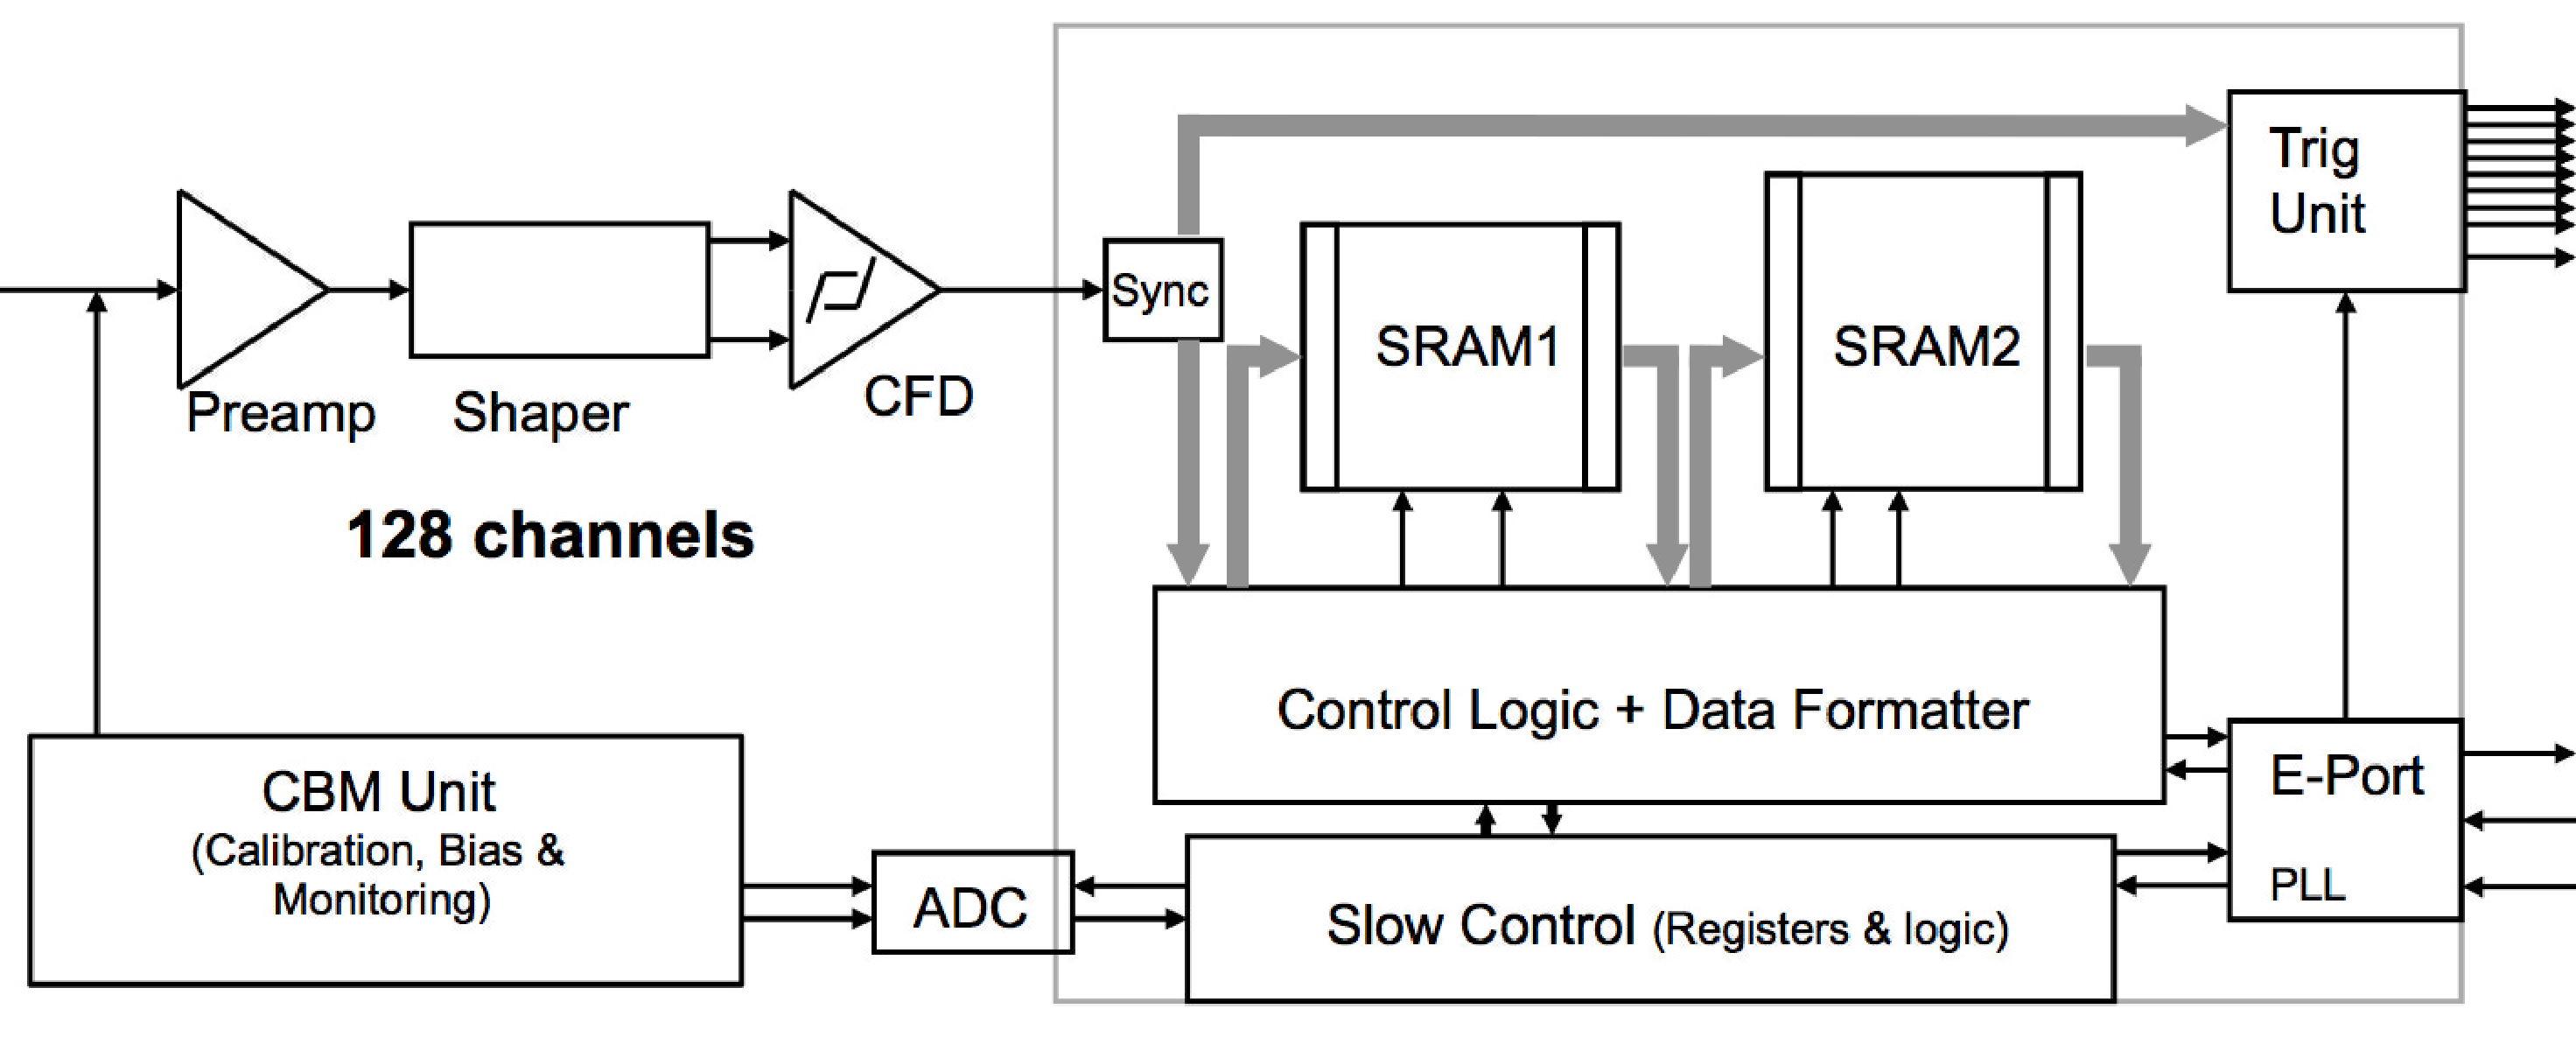
\includegraphics[width=\textwidth]{img/II-2-daq/vfat3.pdf}
        \caption{??? \cite{Colaleo:2021453}.}
        \label{fig:II-2-daq-vfat3}
      \end{figure}

      \paragraph{The analog front-end} is further optimized for the readout of GEMs in particular. It is composed of 128 channels which amplify and shape the analog signals from the strips with programmable shaping times to allow for various integration lengths of the signal. According to the gas mixture, signal charge from the GEM can last for approximatly 60 ns. Increasing the shaping time to fully integrate the charge will result in a higher signal to noise ratio. Simulations performed on the analog front-end show that a time resolution of 7 ns can be achieved by using a Constant Fraction Discriminator (CFD) with a shaping time of 50 ns. After shaping, the amplitude of the analog signal is compared against a programmable threshold by a comparator to yield a binary output flag for each channel. \\

      \paragraph{The fixed latency path} is used to provide a fast hit information to the trigger system of CMS at a frequency equal to the LHC clock of 40 MHz. The trigger unit inside the VFAT3 formats the output of the 128 comparators and transmits it over 8 differential pairs at a rate of 64 bits per BX. It allows to either encode a logical-OR of two adjacent strips effectivly dividing the number of bits to send by a factor two, or use a zero supression algorithm to solely transmit information on hit strips. Ensuring a fixed latency on this path in crucial to maintain predictability in the trigger system and identify the correct BX. \\

      \paragraph{The variable latency path} is activated upon reception of an L1A to transmit the full granularity information on an event that has been accepted by the trigger system. The VFAT3 holds two Static Random-Access Memories (SRAMs) which are used to store events. The SRAM1 is a circular buffer filled at a frequency equal to the LHC clock with the output of the 128 comparators. When the VFAT3 receives an L1A, it transfers a given event from the SRAM1 to the SRAM2 and adds the BX Counter (BC) and the Event Counter (EC), which respectivly count the number of BX elapsed and the number of L1A received, to the event data. To determine which event needs to be transfered, the chip uses a programmable parameter called the latency that informs the system on the delay between the digitization of an event and the arrival of an L1A corresponding to the same event. It is a measures of the response time of the trigger system to a given event which is a fixed delay. Events stored in the SRAM2 are then formated and sent over a single differential pair out of the VFAT3. The formatting of the data can be selected using a programmable register to be either lossless or zero suppressed. \\

      \paragraph{The slow control} module handles the configuration of the internal registers of the VFAT3. These registers define quantities such as the threshold of the analog front-end, the latency, the readout data format, etc. Coupled with the Calibration, Bias \& Monitoring (CBM) unit, it allows to perform calibration routines on the chip. \\

      \paragraph{The fast control} defines all the time sensitive commands that the VFAT3 receives. These are the Event Counter 0 (EC0), Bunch Counter 0 (BC0), Calibration Pulse (CalPulse), Resynchronisation (Resync), and L1A. The EC0 and BC0 commands respectivly reset the EC and BC; the CalPulse is used to send a calibration pulse on given strips in order to callibrate the analog front-end; the ReSync command resets the internal pointers; and the L1A informs the VFAT3 that an event needs to be transfered to the DAQ.

    \subsection{The GEM Electronics Board}

      The limited space in which the GEM detectors will be installed constrains the design of the system by making it impossible to run flat cables for the 24 VFAT3s. Therefore, the GEB, a Printed Circuit Board (PCB) of the same dimension as the GEM detector, was designed to route the signals of the front-end chips to the OH located on the large side of the detector, furthest away from the beam pipe. A picture of a prototype of the GEB is shown on the right in Figure \ref{fig:II-2-daq-geb}. The functions of the GEBs are to host the VFAT3 ASICs connected to the 24 sectors of the GEM readout board, route their signals to the OH, distribute power to the chips, and provide electric shielding to the detector. The GEB is divided into three columns of eight VFAT3s, further divided into two sectors each as represented in the left picture in Figure \ref{fig:II-2-daq-geb}. The clock, slow control, and fast control are commonn for each column. \\

      \begin{figure}[h!]
        \centering
        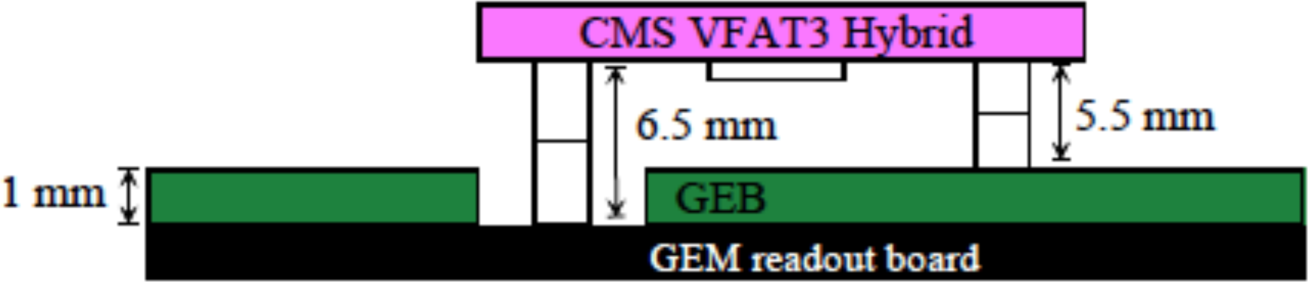
\includegraphics[width=0.8\textwidth]{img/II-2-daq/geb.pdf}
        \caption{??? \cite{Colaleo:2021453}.}
        \label{fig:II-2-daq-geb}
      \end{figure}

      The VFAT3s are soldered on the GEB and connected to the GEM readout board on which it rests through a flexible PCB. The control and data signals from the chips are routed on the PCB towards four connectors located on the large side of the detector which connect to the OH. The power for the VFAT3s and the OH is distributed by the GEB using radition hard DC/DC converters developped by CERN which convert the incoming low voltage to the required voltages. In addition, the bottom layer of the GEB is grouded proving shielding to the detector from external ElectroMagnetic Interference (EMI).

    \subsection{The OptoHybrid}

      The OH is the interface between the VFAT3 ASICs and the off-detector system. It is a 10 cm $ \times $ 20 cm board mounted on the GEB equipped with a Field Programmable Gate Array (FPGA) and Integrated Circuits (ICs) dedicated to the operation of the optical links. The FPGA solely handles the trigger data by applying zero suppression algorithms, formatting the data, and sending it to the CSC and the GEM trigger system separatly over two optical links using the SFP+ connectors. The other functions of the VFAT3s are directly connected to the three GBT chipsets installed on the OH. Each GBT chipset is capable of handling a column of eight VFAT3s.

    \subsection{The GBT and Versatil Link}

      The GBT \cite{Moreira:1235836} and Versatil Link \cite{Soos:1609037} are projects developped by CERN providing radiation hard tools for optical communication to the LHC experiments. The GBT is an optical data link technology providing bidirectionnal 4.8 Gb/s (Gigabits per second) serial communication designed to connect the on-detector and off-detector electronics. It is declined in two version: the GBTX which is a radiation hard ASIC, and the GBT-FPGA which is a core that can be implemented inside an FPGA. Complementary to the GBT which provides the data structure and communication protocol between components, the Versatil Link project develops radiation hard optical transceivers. The integration of the GBTX, Verstil Link, and GBT-FPGA projects is shown in Figure \ref{fig:II-2-daq-gbt-versatile}. \\

      \begin{figure}[h!]
        \centering
        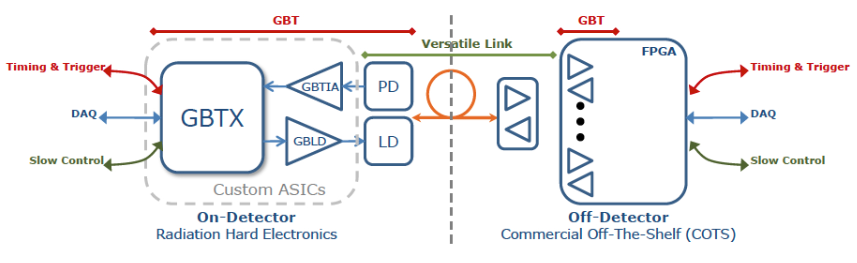
\includegraphics[width=\textwidth]{img/II-2-daq/gbt-versatile.pdf}
        \caption{??? \cite{Moreira:1235836}.}
        \label{fig:II-2-daq-gbt-versatile}
      \end{figure}

      The GBT defines a data format shown in Figure \ref{fig:II-2-daq-gbt-frame}. The stream of data is divided into frames of 120 bits transmitted at 40 MHz, resulting in a data rate of 4.8 Gb/s from which 3.36 Gb/s are accessible by the user. The frame start with a four bits header (H) which defines the frame type and ends with 32 bits of Forward Error Correction (FEC). The error correction is done by encodeding the data using a Reed-Salomon code that can correct bit flips due to radiation. The 84 remaining bits are user accessible. The first two bits are used for internal slow control (IC) and the two following bits for external slow control (EC), leaving 80 bits of data (D) accessible to the user for DAQ, TTC, and slow control purposes. \\

      \begin{figure}[h!]
        \centering
        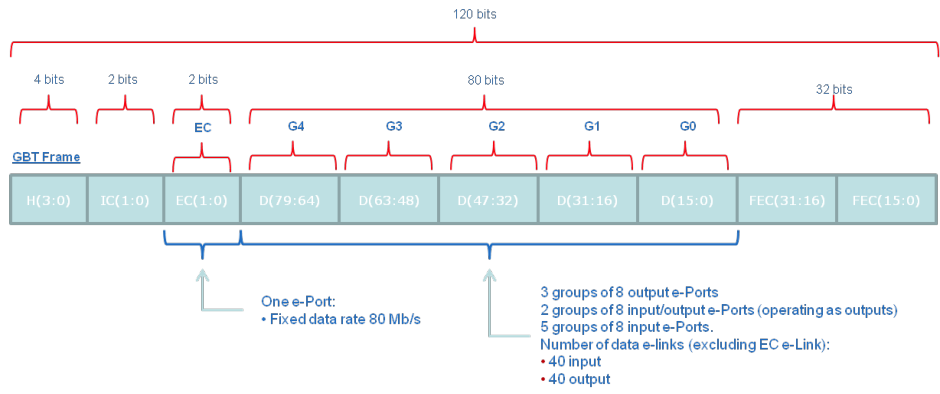
\includegraphics[width=\textwidth]{img/II-2-daq/gbt-frame.pdf}
        \caption{??? \cite{Moreira:1235836}.}
        \label{fig:II-2-daq-gbt-frame}
      \end{figure}

      The header is used to syncrhonize the link by requiering the detection of a series of valid header fields. It is therefore protected by the FEC in order to ensure efficient frame-locking. From the slow control bits, both running at 80 Mb/s, the IC is reserved for the control and monitoring of the GBTX while the EC on the other hand can be freely assigned by the user. The data field is used to transfer DAQ, TTC, and slow control requests to the various subsystems connected to the GBT and can implement any user defined protocol. The FEC uses two Reed-Salomon codes interleaved with 4-bit symbols each capable of correcting double errors. This means that the total frame can recover up to 16 corrupted bits. Additionnaly, the GBT frame is scrambled in order to maintain DC balance on the transmission lines. \\

      On the FPGA side, the communication protocol is seen by the user as a 84-bits-wide vector that is sampled at a frequency of 40 MHz an then formatted by the GBT-FPGA core. The GBTX ASIC on the other hand uses 42 Electric serial Links (E-Links) to handle the data. The structure of the GBTX is shown in Figure \ref{fig:II-2-daq-gbt-asic}. Each E-Link is composed of three differential pairs: one to transmit and one to receive the data, and one to carry the clock synchronuous to the data. From the 42 E-links, one is dedicated to the IC and one to the EC, each transfering data at 80 Mb/s by serializing the two IC or EC bits of the GBT frame on a single link. The use of the remaining 40 E-Links is defined according to the speed at which they operate. The 80-bit-long user data can be configured to either be serialised by a factor two, four, or eight resuling in the use of 40, 20, or 10 E-Links respectivly running at 80 MHz, 160 MHz, or 320 MHz to accomodate the data rate. For the GEM project, a serialisation factor of eight is used, meaning that from the 40 E-Links, only 10 are in used, each of them tranfering 8 bits per BX. \\

      \begin{figure}[h!]
        \centering
        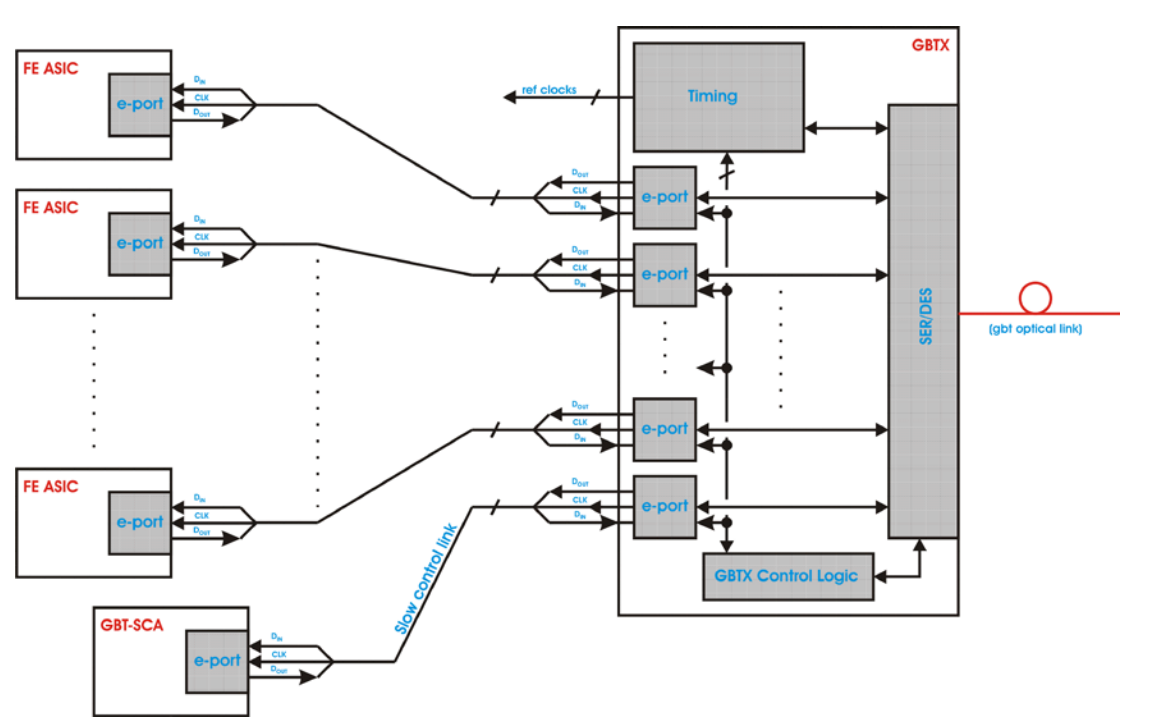
\includegraphics[width=0.8\textwidth]{img/II-2-daq/gbt-asic.png}
        \caption{??? \cite{Moreira:1235836}.}
        \label{fig:II-2-daq-gbt-asic}
      \end{figure}

      To convert the GBTX signals into optical communication, the Versatil Link project provides two laser diode modules: a transceiver module called VTRx and a dual transmitter module called VTTx. The modules have been designed to wistand high magnetic field and radiation doses as encountered in the LHC experiments. The maximal bit rate is of 4.8 Gb/s with a bit error rate inferior to 10$^{-12}$.

    \subsection{The microTCA Standard}

      The off-detector electronics is implemented using the microTCA crate standard to manage the back-end system. The microTCA standard was developped for the telecommunication industry as a successor for the Advanced Telecommunications Computing Architecture (ATCA) technology. It uses a smaller form factor for the AMCs declines into a single width (73.8 mm $ \times $ 181.5 mm) or double width (148.8 mm $ \times $ 181.5 mm) version. The key feature of the crate is the topology of the backplane connecting the AMCs. The latter is not defined in the specifications but often implements a dual-star network which provides reduduncy and thus avoid critical failures of the system upon malfunction of a component. \\

      The structure of the crate is shown in Figure \ref{fig:II-2-daq-utca-crate}. Managment and control of the subsystems of the crate are performed by the MicroTCA Carrier Hub (MCH), which in failure critical systems can be accompagnied by a second MCH for redunduncy. These two MCHs are the central points of the network in dual-star topology. They communicate with the Cooling Units (CUs), Power Modules (PMs), and AMCs through the Intelligent Platform Management Interface (IPMI). The CUs and PMs are equipped with a Enhanced Module Managment Controller (EMMC) and the AMCs with a Module Managnment Controller (MMC) which are used to communicate with the MicroTCA Carrier Management Controller (MCMC) of the MHCs. These controllers implement the IPMI protocol and provide system managment functions to the crate. Upon power-on of the crate or hot-swap of an AMC, the MCHs provide minimal power to the EMMCs and MMCs through dedicated lines in order to start the initial transaction sequence. During this exchange, the power requirements of the modules are defined and a boot-up sequence takes place. Once the transaction is closed, power is provided to the rest of the module and normal operation begins. A power-off sequence takes place when the crate is shutdown or an AMC is removed. 

      \begin{figure}[h!]
        \centering
        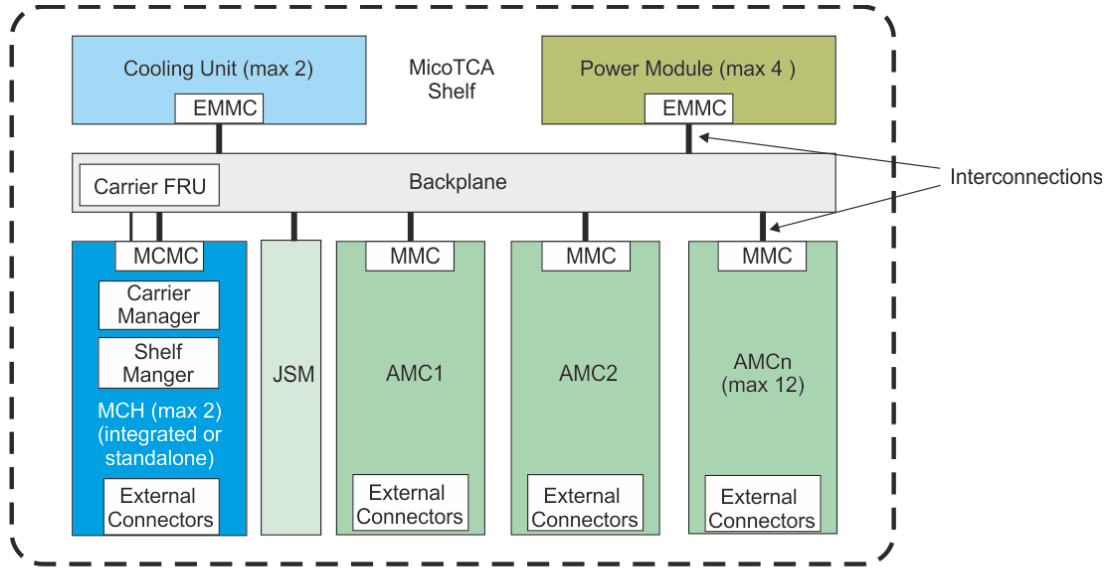
\includegraphics[width=\textwidth]{img/II-2-daq/utca-crate.png}
        \caption{??? \cite{VADATECH}.}
        \label{fig:II-2-daq-utca-crate}
      \end{figure}

    \subsection{The MP7 Advanced Mezzanine Card}

    \subsection{The AMC13}

    \subsection{The IPBus Protocol}

    \subsection{The XDAQ Application}

  \section{The CSC Data Acquisition System}

  \section{The CMS Central Data Acquisition System}






























-
